\documentclass[12pt]{article}
% Common preamble of wellbeing.tex, wellbeing_region.tex and wellbeing_discrepancy.tex
% Compile from papers/:  latexmk -pdf -outdir=build <file>.tex
\usepackage[T1]{fontenc}
\usepackage[utf8]{inputenc}
\usepackage{lmodern}
\usepackage[margin=2.5cm]{geometry}
\usepackage{setspace}
\onehalfspacing
\usepackage{amsmath, amssymb}
\usepackage{graphicx}
\usepackage{booktabs, makecell, threeparttable, adjustbox}
\usepackage{caption}
\captionsetup{font=small, labelfont=bf}
\usepackage[authoryear, round]{natbib}
\bibliographystyle{apalike}
\usepackage{xspace}
\usepackage{xcolor}
\usepackage[colorlinks=true, linkcolor=blue!60!black, citecolor=blue!60!black, urlcolor=blue!60!black]{hyperref}
\usepackage{lineno}
% Placeholders for information to be completed by the author
\newcommand{\todo}[1]{\textcolor{red}{[TODO: #1]}}
% Numbers computed by code_wellbeing/main.R (percentages are given without the % sign)
\newcommand{\corGallupWHR}{0.993\xspace}
\newcommand{\corGallupWHRoldMapping}{0.89\xspace}
\newcommand{\nGallupCountryYears}{2351\xspace}
\newcommand{\nGallupCountries}{168\xspace}
\newcommand{\nWVSCountryYears}{304\xspace}
\newcommand{\nWVSCountries}{108\xspace}
\newcommand{\nWVSRespondents}{439531\xspace}
\newcommand{\nFabre}{11000\xspace}
\newcommand{\nFabreCountries}{10\xspace}
\newcommand{\bestIncome}{Cluster k=7 nominal\xspace}
\newcommand{\shareRegionBetterWVS}{86\xspace}
\newcommand{\shareRegionBetterWVSbest}{79\xspace}
\newcommand{\nSpecsWVS}{952\xspace}
\newcommand{\meanShareIncomeBest}{28\xspace}
\newcommand{\meanRtwoIncomeBest}{19\xspace}
\newcommand{\meanRtwoIncomePPP}{12\xspace}
\newcommand{\meanRtwoRegion}{37\xspace}
\newcommand{\RtwoSatisfiedMeanPPP}{20\xspace}
\newcommand{\RtwoHappinessMeanPPP}{4\xspace}
\newcommand{\RtwoVeryHappyPPP}{0\xspace}
\newcommand{\shareRegionBetterGallup}{35\xspace}
\newcommand{\shareIncomeGallupMean}{60\xspace}
\newcommand{\RtwoGallupMeanPPP}{61\xspace}
\newcommand{\RtwoGallupRegion}{48\xspace}
\newcommand{\RtwoWHRPPP}{63\xspace}
\newcommand{\RtwoWHRRegion}{55\xspace}
\newcommand{\shareRegionBetterNoLatamEE}{27\xspace}
\newcommand{\shareIncomeNoLatamEE}{34\xspace}
\newcommand{\shareRegionBetterContinents}{54\xspace}
\newcommand{\shareRegionBetterWB}{64\xspace}
\newcommand{\cvIncomeSatisfiedMean}{0.18\xspace}
\newcommand{\cvRegionSatisfiedMean}{0.44\xspace}
\newcommand{\cvIncomeGallupMean}{0.60\xspace}
\newcommand{\cvRegionGallupMean}{0.45\xspace}
\newcommand{\shareCvRegionBetterWVS}{100\xspace}
\newcommand{\corHappySatisfied}{0.72\xspace}
\newcommand{\corHappinessSatisfactionMean}{0.76\xspace}
\newcommand{\corVeryHappySatisfiedMean}{0.63\xspace}
\newcommand{\slopeVeryHappy}{0.005\xspace}
\newcommand{\pVeryHappy}{0.85\xspace}
\newcommand{\happiestFirst}{Switzerland\xspace}
\newcommand{\happiestFirstN}{10\xspace}
\newcommand{\happiestSecond}{Mexico\xspace}
\newcommand{\happiestSecondN}{9\xspace}
\newcommand{\happiestThird}{Kyrgyzstan\xspace}
\newcommand{\happiestThirdN}{6\xspace}
\newcommand{\happiestRegionWestern}{24\xspace}
\newcommand{\happiestRegionLatinAmerica}{19\xspace}
\newcommand{\happiestRegionAsia}{16\xspace}
\newcommand{\happiestRegionAfrica}{5\xspace}
\newcommand{\nHappiestCells}{64\xspace}
\newcommand{\treeRegionFirst}{8\xspace}
\newcommand{\withinRtwoSatisfiedMean}{0.22\xspace}
\newcommand{\withinSlopeSatisfiedMean}{1.68\xspace}
\newcommand{\crossSlopeSatisfiedMean}{1.09\xspace}
\newcommand{\withinSlopeVeryHappy}{0.18\xspace}
\newcommand{\pWithinVeryHappy}{0.004\xspace}
\newcommand{\nWithin}{272\xspace}
\newcommand{\RtwoFreedomSatisfaction}{63\xspace}
\newcommand{\shapleyFreedom}{40\xspace}
\newcommand{\shapleyFreedomRegion}{26\xspace}
\newcommand{\shapleyFreedomIncome}{9\xspace}
\newcommand{\RtwoTolerance}{21\xspace}
\newcommand{\RtwoGod}{0\xspace}
\newcommand{\RtwoGrowth}{2\xspace}
\newcommand{\nonresponseSatisfactionWVS}{1.5\xspace}
\newcommand{\nonresponseHappinessWVS}{1.7\xspace}
\newcommand{\corNonresponseGDP}{-0.08\xspace}
\newcommand{\effectLadder}{-0.45\xspace}
\newcommand{\seLadder}{0.05\xspace}
\newcommand{\effectScale}{0.14\xspace}
\newcommand{\seScale}{0.05\xspace}
\newcommand{\effectLadderZeroTen}{-0.46\xspace}
\newcommand{\effectScaleZeroTen}{-0.26\xspace}
\newcommand{\effectLadderSatisfied}{-9\xspace}
\newcommand{\interactionLadderIncome}{-0.004\xspace}
\newcommand{\pInteractionLadderIncome}{0.92\xspace}
\newcommand{\gradientIncomeSatisfaction}{0.69\xspace}
\newcommand{\pHeterogeneityWording}{0.000\xspace}
\newcommand{\chiHeterogeneityWording}{93.4\xspace}
\newcommand{\wordingCHE}{-0.34\xspace}
\newcommand{\wordingDEU}{-0.53\xspace}
\newcommand{\wordingESP}{-1.12\xspace}
\newcommand{\wordingFRA}{-0.50\xspace}
\newcommand{\wordingGBR}{-0.63\xspace}
\newcommand{\wordingITA}{-0.55\xspace}
\newcommand{\wordingJPN}{0.36\xspace}
\newcommand{\wordingPOL}{-0.55\xspace}
\newcommand{\wordingSAU}{-0.79\xspace}
\newcommand{\wordingUSA}{-0.63\xspace}
\newcommand{\wordingMin}{-1.12\xspace}
\newcommand{\wordingMax}{0.36\xspace}
\newcommand{\decompMeanGap}{-0.39\xspace}
\newcommand{\decompMeanQuestion}{-0.71\xspace}
\newcommand{\decompMeanResidual}{0.32\xspace}
\newcommand{\decompShareLevelQuestion}{1.83\xspace}
\newcommand{\decompVarShareQuestion}{-0.20\xspace}
\newcommand{\decompVarShareResidual}{1.20\xspace}
\newcommand{\decompMeanAbsGap}{0.43\xspace}
\newcommand{\decompMeanAbsResidual}{0.64\xspace}
\newcommand{\decompRmsePredictionGallup}{0.73\xspace}
\newcommand{\decompRmseNaive}{0.42\xspace}
\newcommand{\decompMeanGapSat}{-0.05\xspace}
\newcommand{\decompMeanQuestionSat}{-0.11\xspace}
\newcommand{\decompVarShareQuestionSat}{-0.11\xspace}
\newcommand{\decompSdGap}{0.44\xspace}
\newcommand{\decompSdQuestion}{0.45\xspace}
\newcommand{\decompSdResidual}{0.69\xspace}
\newcommand{\decompCorGapQuestion}{-0.20\xspace}
\newcommand{\decompLowMeanGap}{-0.44\xspace}
\newcommand{\decompHighMeanGap}{-0.34\xspace}
\newcommand{\decompLowMeanQuestion}{-0.85\xspace}
\newcommand{\decompHighMeanQuestion}{-0.56\xspace}
\newcommand{\decompLowMeanResidual}{0.17\xspace}
\newcommand{\decompHighMeanResidual}{0.46\xspace}
\newcommand{\decompLowVarShareQuestion}{-0.52\xspace}
\newcommand{\decompHighVarShareQuestion}{0.15\xspace}
\newcommand{\decompLowShareLevelQuestion}{1.42\xspace}
\newcommand{\decompHighShareLevelQuestion}{2.27\xspace}
\newcommand{\decompLowCorGapQuestion}{-0.47\xspace}
\newcommand{\decompHighCorGapQuestion}{0.14\xspace}
\newcommand{\nDecompCountries}{10\xspace}
\newcommand{\nSameYear}{7\xspace}
\newcommand{\nRecent}{4\xspace}
\newcommand{\varShareQuestionSameYear}{-0.27\xspace}
\newcommand{\varShareQuestionRecent}{-0.81\xspace}
\newcommand{\shareLevelQuestionSameYear}{1.60\xspace}
\newcommand{\shareLevelQuestionRecent}{1.19\xspace}
\newcommand{\meanSampleEffectGallup}{0.75\xspace}
\newcommand{\corFabreWHR}{0.75\xspace}
\newcommand{\minSampleEffectGallup}{0.16\xspace}
\newcommand{\maxSampleEffectGallup}{1.24\xspace}
\newcommand{\meanSampleEffectWVS}{0.54\xspace}
\newcommand{\meanFabreGallupZero}{5.93\xspace}
\newcommand{\meanFabreWVSOne}{6.64\xspace}
\newcommand{\sampleEffectUSWVS}{0.49\xspace}
\newcommand{\nCommon}{149\xspace}
\newcommand{\nCommonCountries}{83\xspace}
\newcommand{\RtwoCommonGallup}{0.49\xspace}
\newcommand{\RtwoCommonWVS}{0.11\xspace}
\newcommand{\slopeCommonGallup}{1.76\xspace}
\newcommand{\slopeCommonWVS}{0.77\xspace}
\newcommand{\slopeGapGDP}{1.07\xspace}
\newcommand{\seSlopeGapGDP}{0.16\xspace}
\newcommand{\RtwoGapGDP}{0.31\xspace}
\newcommand{\slopeQuestionGDP}{0.30\xspace}
\newcommand{\seSlopeQuestionGDP}{1.75\xspace}
\newcommand{\RtwoAdjustedWVS}{0.20\xspace}
\newcommand{\shareIncomeCommonGallup}{51\xspace}
\newcommand{\shareIncomeCommonWVS}{15\xspace}

\newcommand{\Rsq}{\ensuremath{R^2}\xspace}
% Switch: show region-specific material (set to false in wellbeing_discrepancy.tex)
\newif\ifshowregion
\showregiontrue

% Combined paper, formatted for the Journal of Economic Psychology (research article: max. 12,000 words including abstract,
% references, tables, figures and appendix; no footnotes on initial submission; p-values with three decimals).
% Compile from papers/:  latexmk -pdf -outdir=build wellbeing.tex

\title{How Well Does GDP per Capita Predict National Well-Being?\\ World Regions, Datasets, and Question Wording\thanks{Data and code: \url{https://github.com/bixiou/wellbeing_gdp_region} \todo{deposit data and code on a public repository (e.g.\ OSF) before acceptance; Gallup data cannot be redistributed}. The survey was approved by the CIRED institutional review board (IRB-CIRED-2025-2) and pre-registered at \href{https://osf.io/7mzn4}{osf.io/7mzn4}. I thank Claudia Senik and participants in the 2024 STATEC Well-being Conference for helpful comments, Armon Rezai and the Vienna University of Economics and Business (WU Wien) for access to the Gallup World Poll data, and Julieta Toffoli for research assistance. This research did not receive any specific grant from funding agencies in the public, commercial, or not-for-profit sectors. Declaration of interest: none.}}
\author{Adrien Fabre\\ \small CNRS, CIRED \todo{postal address}\\ \small \href{mailto:adrien.fabre@cnrs.fr}{adrien.fabre@cnrs.fr}}
\date{\today}

\begin{document}
\maketitle

\begin{abstract}
\noindent Is GDP per capita a good predictor of national well-being? Using all waves of the World Values Survey (WVS, 1981--2022, \nWVSCountries countries), I find that log GDP per capita explains on average \meanRtwoIncomePPP\% of the cross-country variance of eight well-being indicators, and that a country's broad world region is a better predictor, in and out of sample, in \shareRegionBetterWVS\% of \nSpecsWVS specifications. This advantage stems from Latin America and the former Eastern Bloc, and it vanishes in the Gallup World Poll, where income predicts life evaluations as well as region. To understand why the two datasets disagree, I randomize the question wording (Cantril ladder vs.\ life satisfaction) and scale (0--10 vs.\ 1--10) in an online survey of \nFabre respondents in ten high-income countries. The ladder shifts answers by \effectLadder points, with effects varying across countries, which explains why Gallup levels are lower than WVS levels. However, the question effect explains none of the cross-country variation in the Gallup--WVS gap, pointing to differences in samples, modes and context rather than wording.
\end{abstract}
% TODO make all figures conforming to English style, e.g. in the abstract 11,000 instead of 11000 and $-$0.45 instead of -0.45

\noindent\textbf{Keywords:} subjective well-being; life satisfaction; GDP; world regions; survey methodology; question wording.\\
\noindent\textbf{JEL codes:} I31; O15; O57; C83.

% \linenumbers
\section{Introduction}\label{sec:intro}

Which country is the happiest? The answer most often heard, based on the World Happiness Report, is a Scandinavian, high-income country. Behind this answer lies one of the most robust stylized facts of well-being research: across countries, average life evaluations increase with the logarithm of GDP per capita \citep{deaton_income_2008,stevenson_economic_2008,sacks_new_2012}. Using the Gallup World Poll, \citet{deaton_income_2008} finds a correlation above 0.8 between average life evaluation and log GDP per capita; using the World Values Survey (WVS), \citet{inglehart_genes_2000} reported an $R^2$ of about one half for an index of happiness and satisfaction. These correlations are frequently invoked to support the view that economic growth is a reliable route to higher well-being.

This paper revisits the predictive capacity of GDP per capita for national well-being, and asks two questions. First, how much of the cross-country variation in well-being does GDP per capita actually predict, and does it predict it better than a very simple alternative, the country's world region? Second, why do the two main sources of cross-national well-being data, Gallup and the WVS, give different answers to the first question? Previous work has noted that income is more strongly related to Gallup's ladder than to WVS measures \citep{deaton_income_2008}, and that national income is more related to life evaluations than to happiness or emotions \citep{inglehart_development_2008,kahneman_high_2010}. Yet whether the difference between datasets comes from the question asked or from the samples has, to my knowledge, not been tested experimentally.

For the first question, I use all seven waves of the WVS (\nWVSCountryYears country-years), eight indicators of national well-being, and seven income measures, and I compare the variance explained by income and by region using the Shapley (LMG) decomposition of $R^2$ \citep{lindeman_introduction_1980,gromping_estimators_2007} and leave-one-country-out cross-validation. For the second question, I embedded a $2 \times 2$ experiment in an online survey of \nFabre respondents in ten high-income countries, randomizing the wording (Gallup's Cantril ladder vs.\ the WVS life-satisfaction question) and the scale (0--10 vs.\ 1--10). Combining the experiment with Gallup and WVS data for the same countries, I decompose the Gallup--WVS gap into a question effect and a residual reflecting differences in samples, modes, context and time.

The results are threefold. First, in the WVS, GDP per capita is a weak predictor of national well-being: it explains on average \meanRtwoIncomePPP\% of the variance of the eight indicators (\meanRtwoIncomeBest\% with the best income measure), and nothing of the share of very happy people. Region is a better predictor in \shareRegionBetterWVS\% of specifications and, out of sample, for every indicator. Second, this conclusion is fragile in two respects: it is driven by Latin America and the former Eastern Bloc, and it does not hold in Gallup, where income predicts life evaluations as well as or better than region (\RtwoGallupMeanPPP\% vs.\ \RtwoGallupRegion\% of the variance of the mean ladder). % TODO: clarify the parenthesis
Third, the experiment shows that question wording has a sizeable effect on levels---the ladder shifts answers by \effectLadder points, more than the average gap between Gallup and the WVS---and that this effect varies across countries. However, the question effect explains none of the cross-country variation in the Gallup--WVS gap, which is instead attributable to differences between samples in the broad sense. The ladder also does not steepen the income gradient within countries. % TODO clarify last sentence
% TODO not sure you conduct the right exercise for the third point. What you need to do is compare WVS/Gallup data for the latest year available in the 10 countries I surveyed to my survey results: reproduce the analysis (LMG of income vs. region) on these 10 countries using past and new data, compare the income coefficient of the four cases new/old x Gallup/WVS. You should also run a regression on the new data: well-being ~ income * wording * scale: a significant interaction coefficient of wording*income would indicate a wording effect, a nil result would suggest a sample effect. 

The paper contributes to three literatures. It adds to the debate on the relationship between income and well-being across countries and over time \citep{easterlin_does_1974,easterlin_happiness_2010,stevenson_economic_2008,deaton_income_2008,jebb_happiness_2018} by showing that the strength of the cross-country relationship depends on the dataset, and by benchmarking income against regions. It relates to work on regional and cultural differences in well-being, in particular the high well-being of Latin America \citep{graham_paradox_2009,rojas_handbook_2016} and the low well-being of transition countries \citep{guriev_unhappiness_2009}, and on the comparability of well-being across cultures \citep{diener_culture_2000,exton_comparing_2015,senik_french_2014}. Finally, it contributes to the methodological literature on the measurement of subjective well-being \citep{kahneman_developments_2006,oecd_guidelines_2013,stone_subjective_2013,bond_sad_2019,kaiser_scientific_2022}, and specifically on the comparability of the Cantril ladder and life-satisfaction questions \citep{bjornskov_how_2010,nilsson_cantril_2024} and on context and mode effects \citep{deaton_understanding_2016,dolan_happy_2016}, by providing experimental estimates of wording and scale effects in ten countries.

Section~\ref{sec:data} presents the data. Section~\ref{sec:region} compares income and region as predictors of national well-being. Section~\ref{sec:discrepancy} investigates the discrepancy between Gallup and the WVS. Section~\ref{sec:discussion} discusses limitations, and Section~\ref{sec:conclusion} concludes.

\section{Data}\label{sec:data}
% Shared section: data on national well-being, income and regions (WVS, Gallup, WHR, WDI)
\subsection{World Values Survey}\label{subsec:wvs}

The World Values Survey (WVS) is the longest-running cross-national survey of values and subjective well-being. I use the WVS time-series file \citep{wvs_trend_2022}, which pools the seven waves conducted between 1981 and 2022: \nWVSRespondents respondents in \nWVSCountryYears country-years and \nWVSCountries countries. National samples are designed to be representative of the adult population, typically with 1,000 to 3,000 respondents, and most interviews are conducted face-to-face (though some recent national surveys used web, mail or mixed modes, e.g. the United States in 2017 and Japan in 2019). All statistics use the survey weights provided by the WVS.

The WVS contains two questions on subjective well-being:
\begin{itemize}
    \item \textit{Happiness}: ``Taking all things together, would you say you are: \textit{Very happy}; \textit{Quite happy}; \textit{Not very happy}; \textit{Not at all happy}.''
    \item \textit{Life satisfaction}: ``All things considered, how satisfied are you with your life as a whole these days?'', answered on a scale from 1 (\textit{Completely dissatisfied}) to 10 (\textit{Completely satisfied}).
\end{itemize}
Non-responses are rare (\nonresponseSatisfactionWVS\% for satisfaction and \nonresponseHappinessWVS\% for happiness on average) and uncorrelated with GDP per capita (correlation: \corNonresponseGDP); they are excluded.

\ifshowregion
\paragraph{Indicators of national well-being.}
Because there is no consensus on how to aggregate ordinal answers into a national indicator, and because the ranking of countries can depend on this choice \citep{bond_sad_2019}, I compute eight indicators for each country-year: % TODO itemize the list below
\textit{Happy} (share answering \textit{Quite} or \textit{Very happy}); \textit{Very Happy}; \textit{Very Unhappy} (share \textit{Not at all happy}); \textit{V.~Happy -- V.~Unhappy} (difference of the two previous shares); \textit{Happiness (mean)} (answers coded $+3$, $+1$, $-1$, $-3$); \textit{Satisfaction (mean)}; \textit{Satisfied} (share answering 6 to 10); and \textit{Happy + Satisfied} (average of \textit{Happy} and \textit{Satisfied}), the index used by \citet{inglehart_genes_2000}. I also compute the share of people whose satisfaction is below 60\% of the national mean, by analogy with relative poverty lines. The indicators are positively but imperfectly correlated: across country-years, the correlation between \textit{Happy} and \textit{Satisfied} is \corHappySatisfied, and between \textit{Very Happy} and \textit{Satisfaction (mean)} it is only \corVeryHappySatisfiedMean.
\fi

\subsection{Gallup World Poll and World Happiness Report}\label{subsec:gallup}

The Gallup World Poll interviews around 1,000 adults per country and year in more than 140 countries, by telephone where coverage is high (typically in high-income countries) and face-to-face elsewhere \citep{gallup_methodology_2022}. Its life-evaluation question is the Cantril ladder \citep{cantril_pattern_1965}: ``Please imagine a ladder, with steps numbered from 0 at the bottom to 10 at the top. The top of the ladder represents the best possible life for you and the bottom of the ladder represents the worst possible life for you. On which step of the ladder would you say you personally feel you stand at this time?''

I use the distribution of answers by country and wave, tabulated from the Gallup World Poll microdata (\nGallupCountryYears country-years, \nGallupCountries countries, 2006--2023), from which I compute the same satisfaction indicators as for the WVS (mean, shares answering 6--10, 8--10, 9--10, 10, 0--4 and 0--2). % TODO shares answering 8--10, 9--10, 10, 0--4 and 0--2 were not mentioned for WVS: make this consistent
These distributions are unweighted. % Gallup's wave $w$ corresponds to year $w+2005$: with this mapping, three-year averages of the ladder computed from these distributions correlate at \corGallupWHR with the (weighted) three-year averages published in the World Happiness Report, against \corGallupWHRoldMapping with the mapping used in earlier versions of this project (year $w+2000$). 
To cover the most recent years, I also use the ladder means published in the World Happiness Report 2026 \citep{whr_2026}, which average Gallup data over three years up to 2023--2025.

\subsection{Income}\label{subsec:income}

My benchmark income measure is the log of GDP per capita at purchasing power parity (PPP, constant 2021 international dollars) from the World Development Indicators \citep{worldbank_wdi_2026}. As an alternative, I use GDP per capita at market exchange rates (constant 2015 US dollars). Missing values are filled in automatically, in three steps: (i) PPP series, which start in 1990, are extended backwards (and gaps filled) using the growth rate of real GDP per capita; (ii) for countries absent from the World Bank data (e.g. Taiwan, or Venezuela in recent years), I use the IMF World Economic Outlook \citep{imf_weo_2026}, converted into constant dollars using the U.S. ratio between the World Bank and IMF series; % TODO clarify what the US ratio is
(iii) remaining gaps are filled with the closest year available (Montenegro 1996). Territories without national accounts use the GDP of the closest entity (e.g. the United Kingdom for Northern Ireland). A robustness check excludes all imputed values.

\ifshowregion
Since one could argue that it is flawed to compare a categorical variable (\textit{region}) with a continuous one (\textit{income}), % TODO improve wording
I also use discrete income indicators, computed within each estimation sample: % TODO clarify what "within each estimation sample" means
income sextiles and income clusters obtained by $k$-means clustering of log GDP per capita, with $k = 5$, 6 or 7. The clusters let the data choose the thresholds between income groups and allow for non-linear relationships, at the cost of more parameters than the log-linear specification.
\fi

\ifshowregion
\subsection{Regions}\label{subsec:regions}

My main classification groups countries into five world regions inspired by the UN regional groups: % TODO why is it "inspired" by UN grouping? what differs from it? if nothing differs, fix wording; otherwise, state what differs
\textit{Africa}, \textit{Asia} (including the Middle East and Central Asia), \textit{Eastern Europe} (the former Eastern Bloc, excluding Central Asia), \textit{Latin America} (including the Caribbean), and \textit{Western} countries (Western Europe, North America, Australia, New Zealand, and Turkey). For robustness, I use four alternative classifications: a six-region variant separating the Middle East and grouping Central Asia with the former Eastern Bloc; the seven World Bank regions; the five continents; and the UN geoscheme sub-regions (about twenty groups).
% TODO show the map of the presentation
\fi

% Shared section: the Fabre (2025) survey experiment
\subsection{A survey experiment on question wording and scale}\label{subsec:fabre}

% TODO add a sentence at the beginning explaining how WVS and Gallup differ
Gallup and WVS differ in two respects that could explain why they disagree: the question (the Cantril ladder on a 0--10 scale vs.\ life satisfaction on a 1--10 scale) and everything else---sampling frames, interview modes, questionnaire context, translations, and survey years. To separate the two, I embedded a randomized experiment in an original survey \citep{fabre_public_2025}. The survey was conducted online between April 15 and July 3, 2025, by Bilendi (or Kantar in Saudi Arabia) on \nFabre respondents in \nFabreCountries high-income countries: the United States (3,000), Japan (2,000), Saudi Arabia (1,000), Germany (1,048), the United Kingdom (826), France (798), Italy (756), Spain (603), Poland (500) and Switzerland (469).\footnote{The survey also covered Russia, where the well-being question was censored.} Samples were stratified with quotas on gender, age, income, education, region and urbanicity,\footnote{Quota variables also included race in the U.S. and citizenship in Saudi Arabia.} and results are reweighted to match population frequencies along these dimensions (with weights trimmed between 0.25 and 4). %Respondents failing an attention test or completing the questionnaire in less than 6 minutes were excluded. The project was approved by the CIRED institutional review board (IRB-CIRED-2025-2) and pre-registered at the Open Science Framework (\href{https://osf.io/7mzn4}{osf.io/7mzn4}).

Toward the end of the questionnaire, after questions on global policies, each respondent was randomly assigned to one of four versions of the life-evaluation question:
\begin{itemize}
    \item \textit{Ladder 0--10} (Gallup's original): the Cantril ladder question quoted in Section~\ref{subsec:gallup}, with steps numbered from 0 (\textit{Worst possible}) to 10 (\textit{Best possible});
    \item \textit{Ladder 1--10}: same wording, with steps numbered from 1 to 10;
    \item \textit{Satisfaction 0--10}: the WVS question quoted in Section~\ref{subsec:wvs}, with answers from 0 (\textit{Completely dissatisfied}) to 10 (\textit{Completely satisfied});
    \item \textit{Satisfaction 1--10} (WVS's original): same wording, with answers from 1 to 10.
\end{itemize}
This $2 \times 2$ design identifies the effect of wording (ladder vs.\ satisfaction) and scale (0--10 vs.\ 1--10), and their interaction, holding the sample, mode, context and time constant. Within each country, the four branches are balanced (each receives between around 25\% % 21\% and 30\% 
of respondents).


\section{Income and region as predictors of national well-being}\label{sec:region}
% Shared section: income, region and national well-being (method and results)
\subsection{Empirical strategy}\label{subsec:method_region}

For each well-being indicator $y$ and each income indicator $x$, I estimate three linear regressions across country-years $i$:
\begin{align} % TODO use notations close to the presentation's
    y_i &= \alpha_1 + \beta_1\, x_i + u_i \label{eq:income}\\
    y_i &= \alpha_2 + \gamma_2' R_i + e_i \label{eq:region}\\
    y_i &= \alpha_3 + \beta_3\, x_i + \gamma_3' R_i + \varepsilon_i \label{eq:both}
\end{align}
where $R_i$ is a vector of region dummies. Denoting $R^2_1$, $R^2_2$ and $R^2_3$ their coefficients of determination, the share of the variance explained by income alone is $R^2_1$. To compare income and region, I decompose $R^2_3$ between the two regressors following \citet{lindeman_introduction_1980} (LMG), i.e.\ using the Shapley value \citep{gromping_estimators_2007}. With two (groups of) regressors, the LMG contribution of income is the average of its contribution when entered first ($R^2_1$) and when entered second ($R^2_3 - R^2_2$). The \textit{share of explained variance due to income} is therefore
\begin{equation}
    s = \frac{R^2_1 + (R^2_3 - R^2_2)}{2\, R^2_3}, \label{eq:share}
\end{equation}
and region is the better predictor whenever $s < 50\%$.

Two features of this comparison could favor region. First, region has four degrees of freedom while log GDP has one. Second, the regions were not chosen blindly. To address the first concern, I report adjusted $R^2$ and, more directly relevant to the question of \textit{predictive} capacity, leave-one-country-out cross-validated $R^2$: each country's observations are predicted by a model estimated on all other countries, and the out-of-sample $R^2$ is one minus the ratio of the sum of squared prediction errors to the total sum of squares. To address the second concern, I report results for four alternative classifications. Other robustness checks include each WVS wave separately, weighting countries by their population, keeping only the last observation of each country, excluding the pandemic years 2020--2021, excluding imputed GDP values, using the previous vintage of GDP data (PPP in constant 2017 dollars), and excluding Latin America and Eastern Europe.

\subsection{Income explains a small share of national well-being in the WVS}\label{subsec:r2_income}

Figure~\ref{fig:satisfaction_gdp} plots mean life satisfaction against GDP per capita for all WVS country-years. The relationship is positive, but the dispersion at any given income level is large: countries with a GDP per capita around 10,000 dollars span most of the range of observed life satisfaction, from the former Soviet republics at the bottom to Latin American countries at the top. Log GDP per capita explains \RtwoSatisfiedMeanPPP\% of the variance of mean satisfaction.

\begin{figure}[htbp]
    \centering
    \caption{Mean life satisfaction vs.\ GDP per capita (PPP), WVS 1981--2022}\label{fig:satisfaction_gdp}
    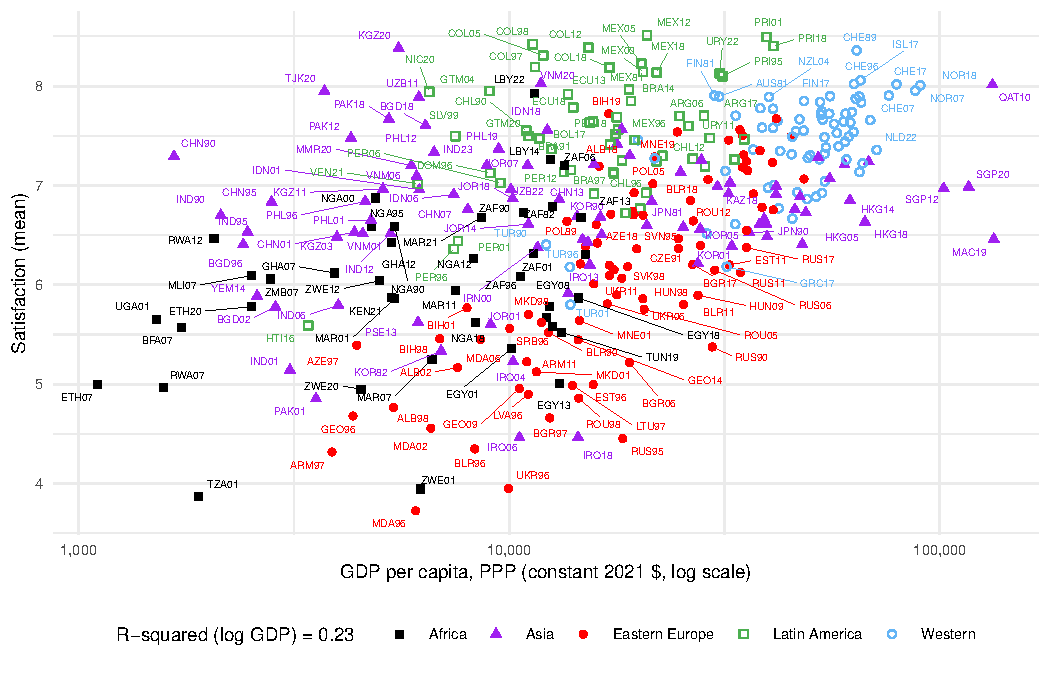
\includegraphics[width=.95\textwidth]{../figures/main/wvs_satisfied_mean_vs_gdp_ppp.pdf}
    \begin{minipage}{.95\textwidth}\footnotesize \textit{Note:} Each point is a country-year (label: ISO code and last two digits of the year). The legend gives the $R^2$ of the regression on log GDP per capita.\end{minipage}
\end{figure}

Table~\ref{tab:r2_income} generalizes this result to all indicators and income measures. On average over the eight indicators, log GDP per capita at PPP explains \meanRtwoIncomePPP\% of the variance, and the best-performing income measure (\bestIncome) explains \meanRtwoIncomeBest\%. The indicators are positively but imperfectly correlated (Appendix Table~\ref{tab:correlation}), and satisfaction-based indicators are better explained than happiness-based ones: log GDP explains \RtwoHappinessMeanPPP\% of the variance of mean happiness and essentially none of the share of \textit{Very happy} people, whose slope with respect to log GDP is statistically indistinguishable from zero (slope \slopeVeryHappy, $p = \pVeryHappy$; Appendix Table~\ref{tab:slopes}). This confirms the observation of \citet{deaton_income_2008} and \citet{inglehart_development_2008} that income is more closely related to life evaluation than to happiness. By contrast, region alone explains \meanRtwoRegion\% of the variance on average (last column).

\begin{table}[htbp]
    \centering
    \caption{Share of the variance of national well-being explained by income alone ($R^2$), WVS 1981--2022}\label{tab:r2_income}
    \begin{adjustbox}{max width=\textwidth}
    \begin{tabular}{lcccccccc}
\toprule
Well-being indicator & \multicolumn{2}{c}{log GDP p.c.} & Sextile & \multicolumn{4}{c}{Income cluster} \\ & PPP & nominal & PPP & $k$=5 PPP & $k$=6 PPP & $k$=7 PPP & $k$=7 nominal & Region \\
\midrule
Happy & 0.13 & 0.18 & 0.20 & 0.19 & 0.19 & 0.20 & 0.23 & 0.36 \\
Very Happy & 0.00 & 0.00 & 0.03 & 0.02 & 0.03 & 0.04 & 0.03 & 0.35 \\
Very Unhappy & 0.06 & 0.09 & 0.12 & 0.11 & 0.13 & 0.13 & 0.14 & 0.16 \\
V. Happy -- V. Unhappy & 0.00 & 0.01 & 0.05 & 0.03 & 0.04 & 0.05 & 0.04 & 0.36 \\
Happiness (mean) & 0.04 & 0.07 & 0.10 & 0.08 & 0.09 & 0.10 & 0.10 & 0.38 \\
Satisfaction (mean) & 0.20 & 0.26 & 0.21 & 0.19 & 0.19 & 0.21 & 0.26 & 0.48 \\
Satisfied & 0.28 & 0.35 & 0.30 & 0.28 & 0.28 & 0.30 & 0.35 & 0.45 \\
Happy + Satisfied & 0.25 & 0.32 & 0.28 & 0.27 & 0.27 & 0.29 & 0.33 & 0.46 \\
\midrule
Mean & 0.12 & 0.16 & 0.16 & 0.15 & 0.15 & 0.17 & 0.19 & 0.37 \\
Max & 0.28 & 0.35 & 0.30 & 0.28 & 0.28 & 0.30 & 0.35 & 0.48 \\
\bottomrule
\end{tabular}

    \end{adjustbox}
    \begin{minipage}{\textwidth}\footnotesize \textit{Note:} $R^2$ of the regression of each well-being indicator (rows) on each income indicator (columns), over \nWVSCountryYears WVS country-years (a few with missing GDP are excluded). The last column gives the $R^2$ of the regression on region dummies.\end{minipage}
\end{table}

\subsection{Region predicts national well-being better than income in the WVS}\label{subsec:region_wvs}

Table~\ref{tab:share_income} reports the share of explained variance due to income, $s$, for each indicator and income measure. It is below 50\% in all cases: on average, the best income measure accounts for \meanShareIncomeBest\% of the variance explained jointly by income and region. The first split of a regression tree using log GDP and region as candidate variables is on region for \treeRegionFirst out of 8 indicators.

\begin{table}[htbp]
    \centering
    \caption{Share of explained variance due to income rather than region (LMG), WVS 1981--2022}\label{tab:share_income}
    \begin{adjustbox}{max width=\textwidth}
    \begin{tabular}{lccccccc}
\toprule
Well-being indicator & \multicolumn{2}{c}{log GDP p.c.} & Sextile & \multicolumn{4}{c}{Income cluster} \\ & PPP & nominal & PPP & $k$=5 PPP & $k$=6 PPP & $k$=7 PPP & $k$=7 nominal \\
\midrule
Happy & 0.22 & 0.29 & 0.31 & 0.30 & 0.30 & 0.32 & 0.34 \\
Very Happy & 0.00 & 0.01 & 0.07 & 0.05 & 0.08 & 0.10 & 0.07 \\
Very Unhappy & 0.22 & 0.31 & 0.41 & 0.38 & 0.43 & 0.44 & 0.45 \\
V. Happy -- V. Unhappy & 0.01 & 0.02 & 0.09 & 0.06 & 0.09 & 0.11 & 0.08 \\
Happiness (mean) & 0.07 & 0.11 & 0.15 & 0.13 & 0.15 & 0.16 & 0.15 \\
Satisfaction (mean) & 0.25 & 0.30 & 0.25 & 0.23 & 0.23 & 0.25 & 0.30 \\
Satisfied & 0.35 & 0.41 & 0.36 & 0.34 & 0.35 & 0.37 & 0.41 \\
Happy + Satisfied & 0.31 & 0.38 & 0.35 & 0.33 & 0.34 & 0.35 & 0.39 \\
\midrule
Mean & 0.18 & 0.23 & 0.25 & 0.23 & 0.25 & 0.26 & 0.28 \\
Max & 0.35 & 0.41 & 0.41 & 0.38 & 0.43 & 0.44 & 0.45 \\
\bottomrule
\end{tabular}

    \end{adjustbox}
    \begin{minipage}{\textwidth}\footnotesize \textit{Note:} Share of the $R^2$ of Equation~\eqref{eq:both} attributed to income by the LMG (Shapley) decomposition, Equation~\eqref{eq:share}. Values below 0.5 indicate that region is the better predictor.\end{minipage}
\end{table}

The result is not an artifact of the larger number of parameters of the region model. Out of sample, region predicts better than income for every indicator (Table~\ref{tab:cv}): for mean satisfaction, the leave-one-country-out $R^2$ is \cvRegionSatisfiedMean with region against \cvIncomeSatisfiedMean with log GDP. For several happiness indicators, income has no out-of-sample predictive power at all (negative cross-validated $R^2$).

\begin{table}[htbp]
    \centering
    \caption{Out-of-sample predictive capacity: leave-one-country-out cross-validated $R^2$}\label{tab:cv}
    \begin{adjustbox}{max width=\textwidth}
    \begin{tabular}{llccccc}
\toprule
Data & Indicator & Obs. & log GDP PPP & Best income variable & Region & log GDP PPP + Region \\
\midrule
WVS, all waves & Happy & 302 & 0.11 & 0.17 & 0.31 & 0.36 \\
WVS, all waves & Very Happy & 302 & -0.03 & -0.06 & 0.29 & 0.29 \\
WVS, all waves & Very Unhappy & 302 & 0.05 & 0.09 & 0.11 & 0.12 \\
WVS, all waves & V. Happy -- V. Unhappy & 302 & -0.02 & -0.05 & 0.30 & 0.29 \\
WVS, all waves & Happiness (mean) & 302 & 0.02 & 0.03 & 0.33 & 0.33 \\
WVS, all waves & Satisfaction (mean) & 302 & 0.18 & 0.19 & 0.44 & 0.51 \\
WVS, all waves & Satisfied & 302 & 0.26 & 0.30 & 0.42 & 0.53 \\
WVS, all waves & Happy + Satisfied & 300 & 0.23 & 0.28 & 0.42 & 0.51 \\
\midrule
WVS, last obs. per country & Happy & 108 & 0.05 & 0.10 & 0.24 & 0.26 \\
WVS, last obs. per country & Very Happy & 108 & -0.01 & -0.04 & 0.25 & 0.24 \\
WVS, last obs. per country & Very Unhappy & 108 & 0.04 & 0.04 & 0.05 & 0.07 \\
WVS, last obs. per country & V. Happy -- V. Unhappy & 108 & -0.02 & -0.06 & 0.25 & 0.24 \\
WVS, last obs. per country & Happiness (mean) & 108 & -0.04 & -0.04 & 0.26 & 0.24 \\
WVS, last obs. per country & Satisfaction (mean) & 108 & 0.13 & 0.12 & 0.36 & 0.40 \\
WVS, last obs. per country & Satisfied & 108 & 0.22 & 0.23 & 0.34 & 0.42 \\
WVS, last obs. per country & Happy + Satisfied & 108 & 0.18 & 0.20 & 0.36 & 0.42 \\
\midrule
Gallup, all years (2006--23) & Satisfaction (mean) & 2344 & 0.61 & 0.66 & 0.49 & 0.68 \\
Gallup, all years (2006--23) & Satisfied & 2344 & 0.65 & 0.72 & 0.52 & 0.72 \\
Gallup, all years (2006--23) & Unsatisfied (0/1--4) & 2344 & 0.63 & 0.65 & 0.48 & 0.68 \\
\midrule
Gallup, last obs. per country & Satisfaction (mean) & 167 & 0.60 & 0.58 & 0.45 & 0.64 \\
Gallup, last obs. per country & Satisfied & 167 & 0.65 & 0.68 & 0.52 & 0.70 \\
Gallup, last obs. per country & Unsatisfied (0/1--4) & 167 & 0.65 & 0.60 & 0.48 & 0.67 \\
\midrule
WHR, 2023--25 average & Satisfaction (mean) & 147 & 0.62 & 0.60 & 0.52 & 0.69 \\
\bottomrule
\end{tabular}

    \end{adjustbox}
    \begin{minipage}{\textwidth}\footnotesize \textit{Note:} Each country's observations are predicted with a model estimated on all other countries. Cross-validated $R^2 = 1 - \sum (y - \hat y_{\text{out-of-sample}})^2 / \sum (y - \bar y)^2$; it can be negative when a model predicts worse than the overall mean.\end{minipage}
\end{table}

Table~\ref{tab:robustness} summarizes \nSpecsWVS estimates (indicator $\times$ income measure $\times$ specification) using the WVS. Region is the better predictor in \shareRegionBetterWVS\% of them (\shareRegionBetterWVSbest\% when restricting to the best income measure). The result holds in each wave except wave 4 (1999--2004, 40 countries), where income and region perform similarly; when countries are weighted by population; when keeping one observation per country; without the pandemic years; without imputed GDP values; with the previous vintage of GDP data; and with the six-region or the UN sub-region classifications.

\begin{table}[htbp]
    \centering
    \caption{Robustness: income vs.\ region across specifications and datasets}\label{tab:robustness}
    \begin{adjustbox}{max width=\textwidth}
    \begin{tabular}{lccccccccc}
\toprule
Specification & Obs. & Countries & \multicolumn{2}{c}{$R^2$ income} & $R^2$ region & \multicolumn{3}{c}{Share of explained variance due to income} & Region better \\ & & & log PPP & best & & log PPP & best & adj. $R^2$ & (share of cases) \\
\midrule
WVS, all waves & 302 & 108 & 0.12 & 0.19 & 0.37 & 0.18 & 0.28 & 0.22 & 1.00 \\
WVS, waves 1--2 (1981--91) & 26 & 21 & 0.07 & 0.43 & 0.58 & 0.09 & 0.40 & 0.10 & 1.00 \\
WVS, wave 3 (1995--99) & 55 & 55 & 0.16 & 0.33 & 0.65 & 0.14 & 0.28 & 0.18 & 1.00 \\
WVS, wave 4 (1999--2004) & 40 & 40 & 0.19 & 0.31 & 0.33 & 0.27 & 0.47 & 0.47 & 0.43 \\
WVS, wave 5 (2004--09) & 58 & 58 & 0.21 & 0.35 & 0.49 & 0.22 & 0.38 & 0.23 & 0.98 \\
WVS, wave 6 (2010--16) & 60 & 60 & 0.08 & 0.22 & 0.27 & 0.14 & 0.41 & 0.19 & 0.96 \\
WVS, wave 7 (2017--22) & 64 & 64 & 0.07 & 0.13 & 0.26 & 0.20 & 0.31 & 0.14 & 1.00 \\
WVS, wave 7 w/o 2020--21 & 45 & 45 & 0.06 & 0.22 & 0.31 & 0.14 & 0.41 & 0.14 & 0.95 \\
WVS, population-weighted & 302 & 108 & 0.10 & 0.19 & 0.23 & 0.24 & 0.44 & 0.33 & 0.84 \\
WVS, last obs. per country & 108 & 108 & 0.10 & 0.18 & 0.33 & 0.18 & 0.32 & 0.21 & 0.96 \\
WVS, no GDP imputation & 283 & 104 & 0.12 & 0.19 & 0.38 & 0.17 & 0.28 & 0.21 & 1.00 \\
WVS, GDP PPP 2017 \$ (old) & 302 & 108 & 0.13 & 0.19 & 0.37 & 0.19 & 0.28 & 0.22 & 1.00 \\
WVS, w/o Latin Am. \& E. Europe & 185 & 68 & 0.16 & 0.27 & 0.18 & 0.34 & 0.68 & 0.54 & 0.27 \\
WVS, 6 regions & 302 & 108 & 0.12 & 0.19 & 0.35 & 0.18 & 0.28 & 0.22 & 1.00 \\
WVS, World Bank regions (7) & 302 & 108 & 0.12 & 0.19 & 0.22 & 0.31 & 0.43 & 0.38 & 0.64 \\
WVS, continents (5) & 302 & 108 & 0.12 & 0.19 & 0.20 & 0.34 & 0.46 & 0.41 & 0.54 \\
WVS, UN sub-regions & 302 & 108 & 0.12 & 0.19 & 0.40 & 0.20 & 0.29 & 0.25 & 1.00 \\
\midrule
Gallup, all years (2006--23) & 2344 & 167 & 0.42 & 0.48 & 0.42 & 0.46 & 0.51 & 0.49 & 0.31 \\
Gallup, last obs. per country & 167 & 167 & 0.42 & 0.44 & 0.41 & 0.44 & 0.48 & 0.45 & 0.37 \\
Gallup, last obs., WVS countries & 105 & 105 & 0.43 & 0.46 & 0.42 & 0.46 & 0.49 & 0.47 & 0.37 \\
Gallup, last obs., 6 regions & 167 & 167 & 0.42 & 0.44 & 0.42 & 0.43 & 0.46 & 0.44 & 0.41 \\
Gallup, last obs., WB regions & 167 & 167 & 0.42 & 0.44 & 0.38 & 0.47 & 0.50 & 0.48 & 0.29 \\
WHR, 2023--25 average & 147 & 147 & 0.63 & 0.63 & 0.55 & 0.56 & 0.56 & 0.56 & 0.00 \\
\bottomrule
\end{tabular}

    \end{adjustbox}
    \begin{minipage}{\textwidth}\footnotesize \textit{Note:} Averages over well-being indicators (8 for the WVS; 7 satisfaction indicators for Gallup; mean ladder for the WHR). ``Best'' refers to the income measure with the highest average $R^2$ in the main WVS specification (\bestIncome). ``Region better'' is the share of indicator $\times$ income-measure combinations for which $s < 0.5$.\end{minipage}
\end{table}

\subsection{Where the region advantage comes from}\label{subsec:region_limits}

Three results qualify this conclusion. First, the advantage of region is driven by two well-known ``anomalies'': Latin America, happier than its income would predict \citep{graham_paradox_2009,rojas_handbook_2016}, and the former Eastern Bloc, unhappier \citep{guriev_unhappiness_2009}. Excluding these two regions, region is the better predictor in only \shareRegionBetterNoLatamEE\% of cases. Second, the result depends on the granularity and design of the classification: with continents or World Bank regions, which do not isolate Latin America or the former Eastern Bloc, region is better in \shareRegionBetterContinents\% and \shareRegionBetterWB\% of cases, respectively. Third, and most importantly, the conclusion does not carry over to Gallup data. In Gallup's latest observation for each of \nGallupCountries countries, log GDP explains \RtwoGallupMeanPPP\% of the variance of the mean ladder, against \RtwoGallupRegion\% for region, and income accounts for \shareIncomeGallupMean\% of the explained variance (Appendix Table~\ref{tab:share_gallup}). Over all Gallup specifications, region is the better predictor in only \shareRegionBetterGallup\% of cases, mostly for indicators of the upper tail of the distribution (shares answering 9--10 or 10), which are almost unrelated to income. With the latest WHR data (2023--2025), log GDP explains \RtwoWHRPPP\% of the variance of the ladder against \RtwoWHRRegion\% for region.

The relation between GDP and well-being is thus much weaker in the WVS than in Gallup. The same holds when restricting both datasets to the \nCommon country-years observed by both surveys: the $R^2$ of mean life evaluation on log GDP is \RtwoCommonGallup in Gallup and \RtwoCommonWVS in the WVS. Whether ``GDP is a poor predictor of national well-being'' therefore depends on which of the two datasets one trusts.

\subsection{Other correlates and within-country evidence}\label{subsec:correlates}

What do regions capture? Appendix Table~\ref{tab:correlates} decomposes the variance of mean satisfaction among income, region and one additional country-level variable from the WVS. The average perceived freedom of choice and control over one's life (``how much freedom of choice and control you feel you have over the way your life turns out'') alone explains \RtwoFreedomSatisfaction\% of the variance of mean satisfaction; in a Shapley decomposition with income and region, it accounts for \shapleyFreedom percentage points, against \shapleyFreedomRegion for region and \shapleyFreedomIncome for income. This variable is itself a subjective evaluation, so this correlation should not be read causally, but it suggests that non-material dimensions of life are central to regional differences \citep{inglehart_development_2008}. Tolerance of homosexuality (\RtwoTolerance\%), the importance of God (\RtwoGod\%) and GDP growth over the previous five years (\RtwoGrowth\%) explain much less.

Finally, the cross-sectional relation should not be confused with the relation over time. Within countries (country fixed effects, \nWithin observations from countries surveyed at least twice), mean satisfaction increases with log GDP per capita, with a slope of \withinSlopeSatisfiedMean per unit of $\log_{10}$ GDP (i.e.\ per tenfold increase), larger than the cross-sectional slope (\crossSlopeSatisfiedMean), and even the share of \textit{Very happy} people increases (slope \withinSlopeVeryHappy, $p = \pWithinVeryHappy$). Income growth explains \withinRtwoSatisfiedMean of the within-country variance (Appendix Table~\ref{tab:within}). These within-country associations are consistent with \citet{stevenson_economic_2008} and \citet{sacks_new_2012} rather than with a strict version of the Easterlin paradox \citep{easterlin_does_1974,easterlin_happiness_2010}, although they may reflect common shocks (e.g.\ transition recessions) rather than the effect of income per se.

\subsection{What are the happiest countries?}\label{subsec:happiest}

Rankings of countries depend on the indicator. Taking, for each indicator and each wave (and all waves combined), the happiest country-year, \happiestFirst appears most often (\happiestFirstN times out of \nHappiestCells), followed by \happiestSecond (\happiestSecondN) and \happiestThird (\happiestThirdN) (Appendix Table~\ref{tab:happiest}). The happiest country-years are Western (\happiestRegionWestern), Latin American (\happiestRegionLatinAmerica), Asian (\happiestRegionAsia) or African (\happiestRegionAfrica). The richest countries are thus not necessarily the happiest: the link between income and well-being seems to be that rich countries rarely experience low well-being, rather than that they reach the highest levels.


\section{Why do Gallup and the WVS disagree? Wording vs.\ samples}\label{sec:discrepancy}
% Shared section: why do Gallup and the WVS disagree? Wording vs. sampling
\subsection{Experimental effects of wording and scale}\label{subsec:experiment}

Table~\ref{tab:fabre_regressions} reports regressions of the answer on the randomized treatments, with country fixed effects, survey weights and heteroskedasticity-robust standard errors. The ladder wording shifts answers by \effectLadder points on average (s.e.\ \seLadder), i.e.\ respondents rate their lives lower on the ``best possible life'' ladder than when asked how satisfied they are. This is in line with evidence that the two questions elicit different considerations: in open-ended answers, the ladder evokes power and wealth more than life satisfaction does \citep{nilsson_cantril_2024}. The scale effect is smaller: answers on the 1--10 scale are \effectScale points higher than on the 0--10 scale (s.e.\ \seScale), which, once the 1--10 answers are linearly stretched to 0--10, amounts to \effectScaleZeroTen points. Wording and scale do not interact. Measured as the share of respondents answering 6 or more, the ladder changes the share ``satisfied'' by \effectLadderSatisfied percentage points.

\begin{table}[htbp]
    \centering
    \caption{Effects of question wording and scale on life evaluation, Fabre (2025) survey experiment}\label{tab:fabre_regressions}
    \begin{adjustbox}{max width=\textwidth}
    
\begingroup
\centering
\begin{tabular}{lcccccc}
   \tabularnewline \midrule \midrule
   Dependent Variables: & \multicolumn{2}{c}{Answer} & Answer (0--10 equiv.) & Satisfied (6+) & \multicolumn{2}{c}{Answer (0--10 equiv.)}\\
   Model:                                                                         & (1)            & (2)            & (3)            & (4)            & (5)            & (6)\\  
   \midrule
   \emph{Variables}\\
   Ladder wording (Gallup)                                                        & -0.451$^{***}$ & -0.455$^{***}$ & -0.456$^{***}$ & -0.088$^{***}$ & -0.464$^{***}$ & -0.494$^{**}$\\   
                                                                                  & (0.046)        & (0.067)        & (0.067)        & (0.013)        & (0.123)        & (0.172)\\   
   Scale 1--10                                                                    & 0.137$^{**}$   & 0.132          & -0.260$^{***}$ & -0.008         & -0.276$^{***}$ & -0.540$^{**}$\\   
                                                                                  & (0.046)        & (0.068)        & (0.072)        & (0.013)        & (0.046)        & (0.182)\\   
   Ladder wording (Gallup) $\times$ Scale 1--10                                   &                & 0.008          & -0.041         & 0.028          &                & 0.055\\   
                                                                                  &                & (0.092)        & (0.097)        & (0.019)        &                & (0.247)\\   
   Income quartile (1--4)                                                         &                &                &                &                & 0.689$^{***}$  & 0.635$^{***}$\\   
                                                                                  &                &                &                &                & (0.031)        & (0.043)\\   
   Income quartile (1--4) $\times$ Ladder wording (Gallup)                        &                &                &                &                & -0.004         & 0.009\\   
                                                                                  &                &                &                &                & (0.042)        & (0.058)\\   
   Income quartile (1--4) $\times$ Scale 1--10                                    &                &                &                &                &                & 0.106\\   
                                                                                  &                &                &                &                &                & (0.061)\\   
   Income quartile (1--4) $\times$ Ladder wording (Gallup) $\times$ Scale 1--10   &                &                &                &                &                & -0.022\\   
                                                                                  &                &                &                &                &                & (0.083)\\   
   \midrule
   \emph{Fixed-effects}\\
   Country                                                                        & Yes            & Yes            & Yes            & Yes            & Yes            & Yes\\  
   \midrule
   \emph{Fit statistics}\\
   Observations                                                                   & 11,000         & 11,000         & 11,000         & 11,000         & 11,000         & 11,000\\  
   R$^2$                                                                          & 0.05681        & 0.05681        & 0.05942        & 0.04208        & 0.15976        & 0.16024\\  
   \midrule \midrule
   \multicolumn{7}{l}{\emph{Heteroskedasticity-robust standard-errors in parentheses}}\\
   \multicolumn{7}{l}{\emph{Signif. Codes: ***: 0.001, **: 0.01, *: 0.05}}\\
\end{tabular}
\par\endgroup



    \end{adjustbox}
    \begin{minipage}{\textwidth}\footnotesize \textit{Note:} OLS with country fixed effects, survey weights (normalized within country) and heteroskedasticity-robust standard errors in parentheses. \textit{Ladder wording}: Cantril ladder (vs.\ WVS life satisfaction). \textit{Scale 1--10}: answers from 1 to 10 (vs.\ 0 to 10). In columns 3 and 5, 1--10 answers are linearly rescaled to 0--10. Column 5 interacts the wording with the respondent's income quartile within their country. * $p<.05$, ** $p<.01$, *** $p<.001$.\end{minipage}
\end{table}

Two further results matter for the interpretation of cross-country comparisons. First, the ladder does not steepen the income gradient \textit{within} countries: the interaction between ladder wording and the income quartile is \interactionLadderIncome ($p = \pInteractionLadderIncome$), against a gradient of \gradientIncomeSatisfaction points per quartile (column 5). So, at least among individuals in high-income countries, the ladder is not more ``about money'' than the satisfaction question. Second, the wording effect differs markedly across countries (Figure~\ref{fig:fabre_variants}). It ranges from \wordingMin points (Spain) to \wordingMax (Japan), where the ladder yields \textit{higher} answers than the satisfaction question, and the hypothesis of a common effect across countries is strongly rejected ($\chi^2(9) = \chiHeterogeneityWording$, $p < .001$). Question wording therefore affects not only the level but also the ranking of countries.

\begin{figure}[htbp]
    \centering
    \caption{Mean answer by question variant and country, Fabre (2025)}\label{fig:fabre_variants}
    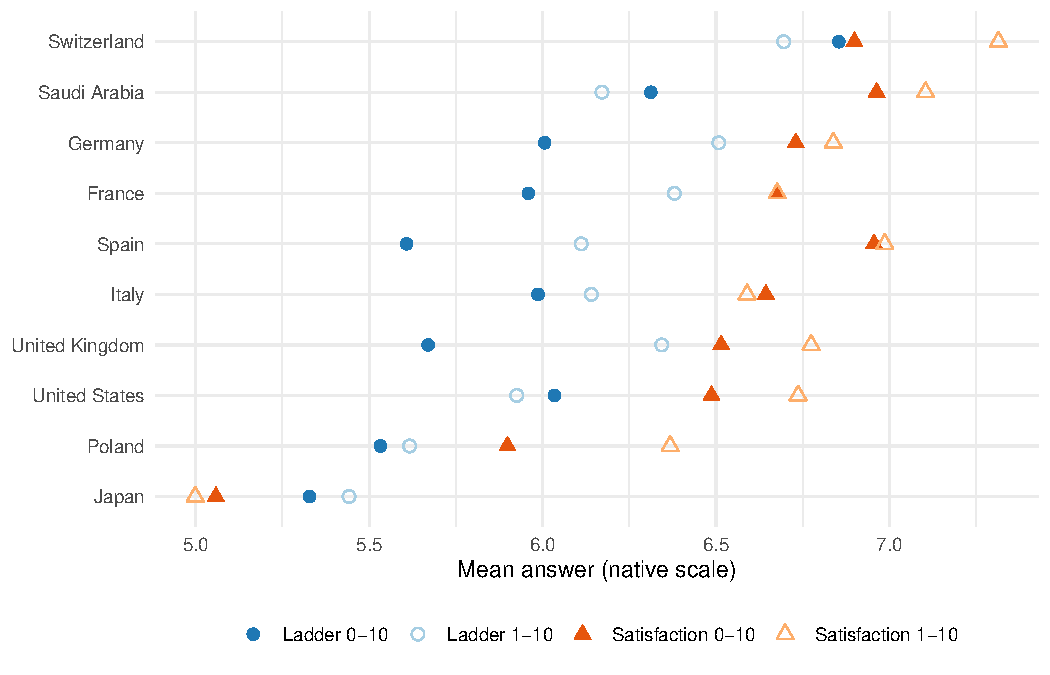
\includegraphics[width=.85\textwidth]{../figures/main/fabre_variants_by_country.pdf}
    \begin{minipage}{.85\textwidth}\footnotesize \textit{Note:} Weighted mean answer on the native scale of each variant (0--10 or 1--10).\end{minipage}
\end{figure}

\subsection{Decomposing the Gallup--WVS gap in ten countries}\label{subsec:decomposition}

For each country $c$ of the experiment, I define the observed gap between Gallup and the WVS as $D_c = G_c - W_c$, where $W_c$ is the mean satisfaction in the latest WVS survey of the country and $G_c$ the mean ladder in Gallup the same year (or the closest year, at most three years apart; seven countries have an exact match). Comparing the two datasets in the same year removes the influence of changes in well-being over time. The experiment measures, within the same sample, the \textit{question effect} $Q_c = F_c(\text{ladder 0--10}) - F_c(\text{satisfaction 1--10})$, where $F_c(v)$ is the mean answer to variant $v$ in country $c$. The residual $R_c = D_c - Q_c$ is the part of the gap due to everything that differs between the two datasets except the question: sampling frames, interview modes, questionnaire context, translations, and survey-specific time effects. This decomposition assumes that the question effect measured online in 2025 applies to the Gallup and WVS samples of earlier years.

Table~\ref{tab:decomposition_country} and Figure~\ref{fig:decomposition} present the decomposition for each country, and Table~\ref{tab:decomposition_summary} summarizes it with 95\% confidence intervals from a bootstrap that resamples respondents in the three surveys. On average, the gap between Gallup and WVS answers is $D = \decompMeanGap$ points. The question effect is even larger in absolute value: $Q = \decompMeanQuestion$ points. Wording (and scale) thus fully account for the fact that Gallup yields lower levels than the WVS in high-income countries, and the residual partly offsets it ($R = \decompMeanResidual$). Since the two components move in opposite directions, another way to summarize the level difference is to compare the size of the two movements: the question accounts for $|\bar Q|/(|\bar Q|+|\bar R|) = \decompShareAbsQuestion$ (95\% CI [\decompLowShareAbsQuestion; \decompHighShareAbsQuestion]) of the gross difference in levels between Gallup and the WVS, and for \decompShareAbsQuestionCountry on average when this share is computed country by country. By this metric, wording is the main driver of the difference in \textit{levels}.

\begin{table}[htbp]
    \centering
    \caption{Decomposition of the Gallup--WVS gap by country}\label{tab:decomposition_country}
    \begin{adjustbox}{max width=\textwidth}
    \begin{tabular}{lllccccccc}
\toprule
Country & Year WVS/EVS (Gallup) & Survey: mode & Gallup & WVS/EVS & Gap $D$ & Ladder 0--10 & Satisf. 1--10 & Question effect $Q$ & Residual $R$ \\ & & & (1) & (2) & (1)$-$(2) & \multicolumn{2}{c}{Fabre (2025)} & & $D-Q$ \\
\midrule
Poland & 2017 & EVS: CAPI & 6.28 & 7.56 & \ensuremath{-}1.28 & 5.53 & 6.37 & \ensuremath{-}0.84 & \ensuremath{-}0.44 \\
Spain & 2017 & EVS: CAPI & 6.47 & 7.49 & \ensuremath{-}1.02 & 5.61 & 6.99 & \ensuremath{-}1.38 & 0.36 \\
Japan & 2019 & WVS: Mail & 5.94 & 6.76 & \ensuremath{-}0.82 & 5.33 & 5.00 & 0.33 & \ensuremath{-}1.15 \\
Italy & 2018 & EVS: CAPI & 6.69 & 7.28 & \ensuremath{-}0.59 & 5.99 & 6.59 & \ensuremath{-}0.60 & 0.01 \\
Germany & 2018 & WVS: CAPI & 7.15 & 7.74 & \ensuremath{-}0.58 & 6.01 & 6.84 & \ensuremath{-}0.83 & 0.25 \\
United Kingdom & 2022 & WVS: CAPI/Web/Mail & 6.76 & 7.32 & \ensuremath{-}0.56 & 5.67 & 6.77 & \ensuremath{-}1.10 & 0.55 \\
France & 2018 & EVS: CAPI & 6.79 & 7.26 & \ensuremath{-}0.47 & 5.96 & 6.68 & \ensuremath{-}0.72 & 0.25 \\
Switzerland & 2017 & EVS: Web/Mail/CAPI & 7.58 & 8.02 & \ensuremath{-}0.43 & 6.85 & 7.31 & \ensuremath{-}0.46 & 0.03 \\
Saudi Arabia & 2003 (2006) & WVS: Face-to-face & 7.06 & 7.28 & \ensuremath{-}0.23 & 6.31 & 7.10 & \ensuremath{-}0.79 & 0.57 \\
United States & 2017 & WVS: Web/Phone & 7.23 & 7.22 & 0.01 & 6.03 & 6.74 & \ensuremath{-}0.70 & 0.71 \\
\bottomrule
\end{tabular}

    \end{adjustbox}
    \begin{minipage}{\textwidth}\footnotesize \textit{Note:} Mean answers on native scales (Gallup: 0--10; WVS: 1--10). The Gallup year is given in parentheses when it differs from the WVS year. WVS mode: main interview mode(s) of the WVS survey (CAPI: computer-assisted personal interviews).\end{minipage}
\end{table}

\begin{figure}[htbp]
    \centering
    \caption{Observed Gallup--WVS gap, question effect and residual by country}\label{fig:decomposition}
    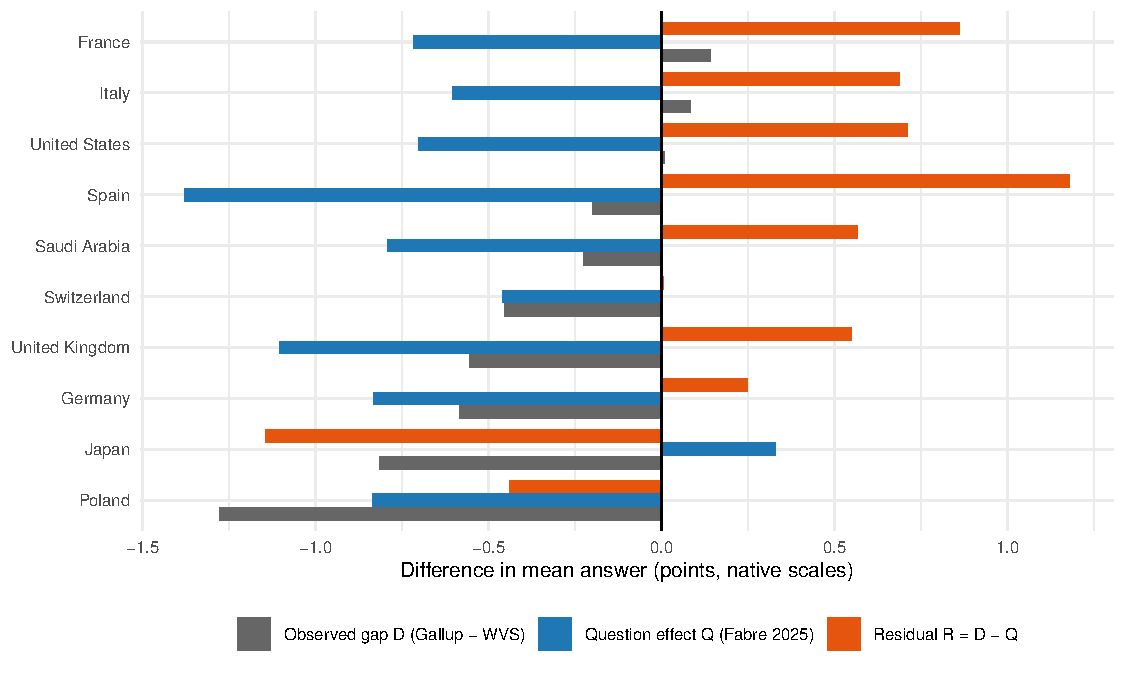
\includegraphics[width=.9\textwidth]{../figures/main/decomposition_by_country.pdf}
\end{figure}

What matters for correlations with GDP and for country rankings, however, is not the level of the gap but its variation across countries, which the previous metrics do not capture: a question effect that shifted all countries by the same amount would score high on them while leaving correlations and rankings unchanged. Here, the question effect explains nothing: the covariance between $D_c$ and $Q_c$ is slightly negative, so that the share of the cross-country variance of the gap attributable to the question, $\mathrm{cov}(D,Q)/\mathrm{var}(D)$, is \decompVarShareQuestion (95\% CI [\decompLowVarShareQuestion; \decompHighVarShareQuestion]), and the residual accounts for the rest. Predicting a country's Gallup score by adding its experimentally measured question effect to its WVS score does worse (root mean squared error: \decompRmsePredictionGallup) than simply adding the average gap (\decompRmseNaive). The conclusion is the same when restricting to the \nSameYear countries where Gallup and WVS are observed the same year (variance share: \varShareQuestionSameYear) or to the \nRecent countries with a WVS survey since 2017 (\varShareQuestionRecent), and for the share of respondents answering 6 or more (\decompVarShareQuestionSat). For instance, the question effect is largest in Spain and the United Kingdom, but the observed gap is small in Spain; Japan is the only country with a positive question effect, but the gap is negative there.

\begin{table}[htbp]
    \centering
    \caption{Decomposition of the Gallup--WVS gap: summary}\label{tab:decomposition_summary}
    \begin{adjustbox}{max width=\textwidth}
    \begin{tabular}{lc}
\toprule
Statistic & Estimate [95\% bootstrap CI] \\
\midrule
Mean gap $D$ (Gallup $-$ WVS) & \ensuremath{-}0.60 [\ensuremath{-}0.64; \ensuremath{-}0.55] \\
Mean question effect $Q$ (wording + scale) & \ensuremath{-}0.71 [\ensuremath{-}0.84; \ensuremath{-}0.56] \\
Mean residual $R$ (sampling, mode, context) & 0.11 [\ensuremath{-}0.04; 0.26] \\
\midrule
Share of mean gap due to question ($\bar Q/\bar D$) & 1.19 [0.94; 1.45] \\
Share of gross level difference due to question ($|\bar Q|/(|\bar Q|+|\bar R|)$) & 0.86 [0.76; 0.99] \\
Same, country average ($\overline{|Q_c|/(|Q_c|+|R_c|)}$) & 0.69 [0.56; 0.72] \\
\midrule
Share of cross-country variance of $D$ due to $Q$ ($\mathrm{cov}(D,Q)/\mathrm{var}(D)$) & 0.11 [\ensuremath{-}0.33; 0.55] \\
Share of cross-country variance of $D$ due to $R$ & 0.89 [0.45; 1.33] \\
Mean absolute gap $|D|$ & 0.60 [0.56; 0.65] \\
Mean absolute residual $|R|$ & 0.43 [0.33; 0.60] \\
Correlation between $D$ and $Q$ & 0.09 [\ensuremath{-}0.26; 0.41] \\
\midrule
Mean gap, share satisfied (6+) & \ensuremath{-}0.07 [\ensuremath{-}0.08; \ensuremath{-}0.06] \\
Mean question effect, share satisfied (6+) & \ensuremath{-}0.11 [\ensuremath{-}0.14; \ensuremath{-}0.08] \\
Variance share due to $Q$, share satisfied & 0.04 [\ensuremath{-}0.33; 0.45] \\
\bottomrule
\end{tabular}

    \end{adjustbox}
    \begin{minipage}{\textwidth}\footnotesize \textit{Note:} \nDecompCountries countries. 95\% confidence intervals from 1,000 bootstrap replications resampling respondents within country $\times$ variant (Fabre), within country (WVS), and answers within country (Gallup, multinomial).\end{minipage}
\end{table}

Two direct comparisons of samples asked the same question corroborate the importance of the residual. First, Gallup respondents (World Happiness Report, 2023--2025) rate their lives \meanSampleEffectGallup points higher on the 0--10 ladder than Fabre (2025) online respondents asked the same question, with differences ranging from \minSampleEffectGallup to \maxSampleEffectGallup across countries. Second, WVS respondents report \meanSampleEffectWVS points higher satisfaction than online respondents asked the WVS question (this comparison also includes changes over time, as WVS surveys are older). These sample (and mode) effects are of the same order of magnitude as the question effect, and they vary across countries. Even in the United States, where the 2017 WVS was itself conducted online, WVS respondents report \sampleEffectUSWVS points higher satisfaction than Fabre (2025) respondents.

\subsection{The global discrepancy}\label{subsec:global_gap}

The ten countries of the experiment are all high-income, whereas the Gallup--WVS discrepancy matters most for the global relation between GDP and well-being. Restricting both datasets to the \nCommon country-years (\nCommonCountries countries) observed by both surveys the same year, log GDP explains \RtwoCommonGallup of the variance of Gallup's mean ladder but only \RtwoCommonWVS of WVS mean satisfaction, and income accounts for \shareIncomeCommonGallup\% of the variance explained jointly with region in Gallup against \shareIncomeCommonWVS\% in the WVS. The gap between the two datasets increases strongly with GDP (Figure~\ref{fig:gap_gdp}): the slope is \slopeGapGDP per unit of $\log_{10}$ GDP (s.e.\ \seSlopeGapGDP, clustered by country), with WVS answers exceeding Gallup answers by around two points in low-income countries, against less than half a point in high-income countries.

\begin{figure}[htbp]
    \centering
    \caption{Gallup ladder minus WVS satisfaction in the same country-year, by GDP per capita}\label{fig:gap_gdp}
    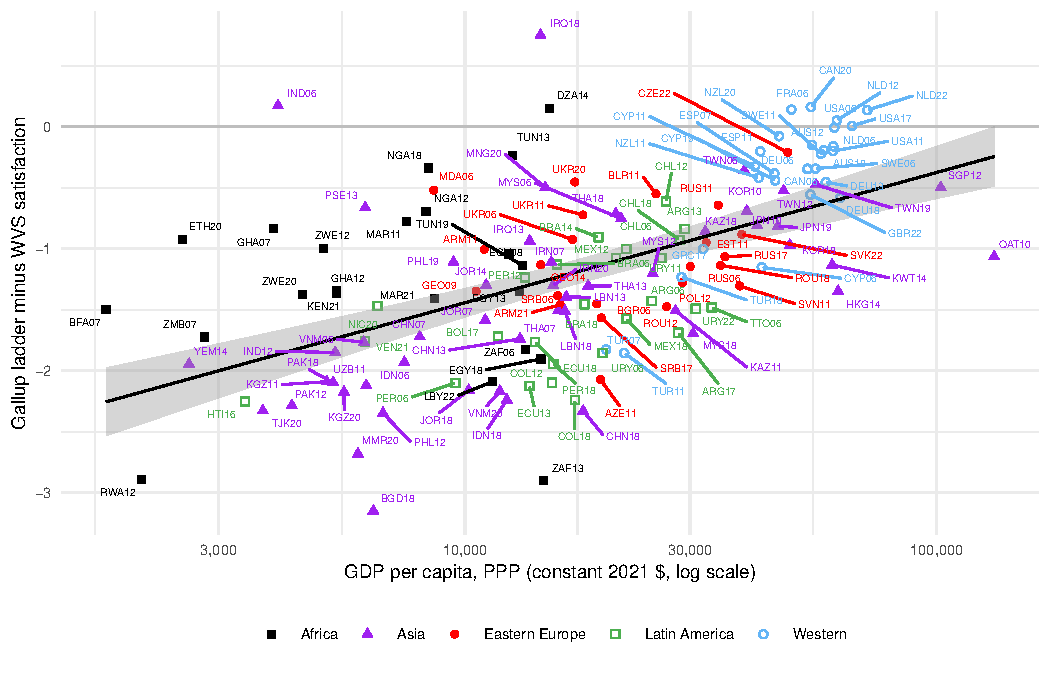
\includegraphics[width=.9\textwidth]{../figures/main/gap_gallup_wvs_vs_gdp.pdf}
    \begin{minipage}{.9\textwidth}\footnotesize \textit{Note:} Mean answers on native scales (Gallup: 0--10; WVS: 1--10), \nCommon country-years observed by both surveys. Line: OLS fit with 95\% confidence band.\end{minipage}
\end{figure}

Could the question explain this pattern? Within the experiment, the question effect is not significantly related to GDP (slope \slopeQuestionGDP, s.e.\ \seSlopeQuestionGDP), which is unsurprising given the narrow range of GDP among the ten countries. Even taking this point estimate at face value and extrapolating it to all countries, adjusting WVS answers for the predicted question effect would raise the $R^2$ of WVS satisfaction on log GDP only from \RtwoCommonWVS to \RtwoAdjustedWVS, far from Gallup's \RtwoCommonGallup. The experiment cannot rule out that the wording effect is much larger in low-income countries---for instance if the ``best possible life'' evokes material comparisons more strongly where material deprivation is widespread---but nothing in the high-income evidence points in that direction: the ladder does not steepen the individual income gradient (Section~\ref{subsec:experiment}), and the country-level question effects are unrelated to the observed gaps.


\section{Discussion}\label{sec:discussion}
\subsection{Income vs.\ region}
% Shared section: interpretation and limitations of the region vs. income analysis
Several caveats apply to the comparison between income and region. First, region is not a mechanism: it bundles culture, history, institutions, social ties, and possibly cross-cultural differences in how people use response scales \citep{chen_response_1995,diener_personality_2003,exton_comparing_2015}. If regional differences partly reflect response styles, then region predicts \textit{measured} well-being without necessarily predicting \textit{experienced} well-being. Existing evidence suggests that self-reported well-being carries information about true well-being \citep{sandvik_subjective_1993,kaiser_scientific_2022}, and studies exploiting migrants suggest that national differences partly reflect a cultural component of well-being rather than mere translation artifacts \citep{senik_french_2014,exton_comparing_2015}, but the present analysis cannot separate these interpretations. Anchoring vignettes \citep{kapteyn_life_2010} or measures of emotional well-being would help.

Second, the advantage of region rests largely on Latin America and the former Eastern Bloc. These are well-documented deviations from the income gradient, but they are not independent of the classification: grouping countries into continents or World Bank regions, which do not isolate these groups, weakens the result. The fairest summary is that GDP per capita leaves much of the cross-country variation unexplained, and that a few large regional deviations explain more of it than income does in the WVS.

Third, the analysis pools country-years that are not independent, and $R^2$ decompositions carry no information on causality. The within-country evidence shows that growth is associated with rising life satisfaction, so the weak cross-sectional relation does not imply that income is irrelevant for well-being.

Fourth, and most importantly, the WVS and Gallup disagree on the strength of the income gradient. In Gallup, income predicts life evaluations about as well as region, or better.

Section~\ref{sec:discrepancy} showed that this discrepancy does not come from the question asked, but from differences between samples in the broad sense.
\subsection{Wording vs.\ samples}
% Shared section: interpretation and limitations of the wording vs. sampling decomposition
The experiment shows that the question matters for levels: the Cantril ladder yields lower answers than the WVS life-satisfaction question, and this difference fully accounts for the lower average level of Gallup data in high-income countries. But the cross-country pattern of the Gallup--WVS gap, which is what drives differences in correlations with GDP and in country rankings, is not explained by the question. It is explained by the residual, i.e.\ by differences between samples in the broad sense: sampling frames, interview modes \citep{dolan_happy_2016,conti_survey_2011}, questionnaire context \citep{deaton_financial_2012,deaton_understanding_2016}, translations, and time.

Several limitations should be kept in mind. First, the experiment covers ten high-income countries, whereas the gap varies most across income levels. The question effect could be different in low- and middle-income countries, where both Gallup and the WVS mostly interview face-to-face; only an experiment in these countries can settle this. Second, the residual lumps together several factors that the design cannot separate. In particular, the question effect was measured with the survey's own translations, toward the end of a questionnaire on global policies, and online; it may differ from the effect that would be obtained with official Gallup and WVS translations, at the beginning of an interview, and face-to-face or by phone. Third, the decomposition assumes that the question effect measured in 2025 applies to earlier years; for several countries, the latest WVS survey dates from the 2000s. Fourth, with ten countries, cross-country statistics are imprecise, as shown by the bootstrap confidence intervals. Finally, online panel respondents report markedly lower well-being than Gallup and WVS respondents asked the same question, a sample and mode effect that deserves attention in its own right as online panels become common in well-being research.


\section{Conclusion}\label{sec:conclusion}

GDP per capita is a weaker predictor of national well-being than is often assumed, but how weak depends on the data. In the WVS, it explains a small share of the cross-country variance of well-being, less than a country's world region, and it explains essentially nothing of the share of very happy people. In the Gallup World Poll, however, income predicts life evaluations as well as region does. A survey experiment in ten high-income countries shows that the question matters for levels---the Cantril ladder yields lower answers than the life-satisfaction question---but that it does not explain the cross-country pattern of the Gallup--WVS gap, which reflects differences in samples, modes, and context.

These findings have two implications. For research, cross-country conclusions about the income--well-being relationship should be checked across datasets, and the choice between Gallup and the WVS should be based on the quality and comparability of their samples rather than on their questions, since wording effects mostly shift levels. Gallup's standardized annual methodology is an argument in its favor for cross-country comparisons, but the gap between datasets is largest in low-income countries, where neither the present experiment nor existing evidence can yet tell which survey is closer to the truth. Replicating the experiment face-to-face in low- and middle-income countries is the natural next step. For policy, the fact that rich countries rarely have low well-being, while many countries at intermediate income levels are as happy as the richest, suggests that growth is neither necessary nor sufficient for high well-being, and that the non-material determinants of well-being that differ across regions deserve more attention in policy evaluation \citep{stiglitz_report_2009,frijters_happy_2020}.

\section*{Declaration of generative AI and AI-assisted technologies in the writing process}
\todo{During the preparation of this work the author used Claude (Anthropic) to write analysis code and draft parts of the manuscript. After using this tool, the author reviewed and edited the content as needed and takes full responsibility for the content of the publication. (Adapt to actual use.)}

\bibliography{wellbeing}

\clearpage
\appendix
\section{Additional results}\label{app:additional}
% Shared appendix: additional results on income, region and national well-being
\renewcommand{\thetable}{A\arabic{table}}
\renewcommand{\thefigure}{A\arabic{figure}}
\setcounter{table}{0}
\setcounter{figure}{0}

\begin{table}[htbp]
    \centering
    \caption{Correlation between national well-being indicators (WVS country-years)}\label{tab:correlation}
    \begin{adjustbox}{max width=\textwidth}
    \begin{tabular}{lcccccccc}
\toprule
& Happy & Very Happy & Very Unhappy & V. Happy -- V. Unhappy & Happiness (mean) & Satisfaction (mean) & Satisfied & Happy + Satisfied \\
\midrule
Happy & 1.00 & 0.61 & -0.73 & 0.70 & 0.90 & 0.72 & 0.72 & 0.90 \\
Very Happy & 0.61 & 1.00 & -0.38 & 0.98 & 0.89 & 0.63 & 0.53 & 0.61 \\
Very Unhappy & -0.73 & -0.38 & 1.00 & -0.55 & -0.68 & -0.57 & -0.57 & -0.68 \\
V. Happy -- V. Unhappy & 0.70 & 0.98 & -0.55 & 1.00 & 0.95 & 0.69 & 0.60 & 0.69 \\
Happiness (mean) & 0.90 & 0.89 & -0.68 & 0.95 & 1.00 & 0.76 & 0.70 & 0.84 \\
Satisfaction (mean) & 0.72 & 0.63 & -0.57 & 0.69 & 0.76 & 1.00 & 0.96 & 0.93 \\
Satisfied & 0.72 & 0.53 & -0.57 & 0.60 & 0.70 & 0.96 & 1.00 & 0.95 \\
Happy + Satisfied & 0.90 & 0.61 & -0.68 & 0.69 & 0.84 & 0.93 & 0.95 & 1.00 \\
\bottomrule
\end{tabular}

    \end{adjustbox}
\end{table}

\begin{table}[htbp]
    \centering
    \caption{Slope of national well-being indicators with respect to $\log_{10}$ GDP per capita (PPP)}\label{tab:slopes}
    \begin{adjustbox}{max width=\textwidth}
    \begin{tabular}{llccccc}
\toprule
Data & Indicator & Slope & s.e. & $p$-value & $R^2$ & Obs. \\
\midrule
WVS & Happy & 0.109 & 0.019 & 0.000 & 0.145 & 337 \\
WVS & Very Happy & 0.003 & 0.025 & 0.915 & 0.000 & 337 \\
WVS & Very Unhappy & \ensuremath{-}0.022 & 0.004 & 0.000 & 0.072 & 337 \\
WVS & V. Happy -- V. Unhappy & 0.024 & 0.026 & 0.356 & 0.004 & 337 \\
WVS & Happiness (mean) & 0.268 & 0.083 & 0.001 & 0.045 & 337 \\
WVS & Satisfaction (mean) & 1.144 & 0.142 & 0.000 & 0.234 & 337 \\
WVS & Satisfied & 0.237 & 0.024 & 0.000 & 0.317 & 337 \\
WVS & Happy + Satisfied & 0.173 & 0.019 & 0.000 & 0.276 & 335 \\
\midrule
Gallup & Satisfied & 0.372 & 0.017 & 0.000 & 0.655 & 2344 \\
Gallup & Very satisfied (8--10) & 0.218 & 0.018 & 0.000 & 0.442 & 2344 \\
Gallup & Extremely satisfied (9--10) & 0.065 & 0.009 & 0.000 & 0.178 & 2344 \\
Gallup & Completely satisfied (10) & 0.012 & 0.005 & 0.008 & 0.015 & 2344 \\
Gallup & Unsatisfied (0/1--4) & \ensuremath{-}0.304 & 0.012 & 0.000 & 0.639 & 2344 \\
Gallup & Dissatisfied (0/1--2) & \ensuremath{-}0.135 & 0.009 & 0.000 & 0.432 & 2344 \\
Gallup & Satisfaction (mean) & 1.779 & 0.083 & 0.000 & 0.611 & 2344 \\
\bottomrule
\end{tabular}

    \end{adjustbox}
    \begin{minipage}{\textwidth}\footnotesize \textit{Note:} OLS across country-years; standard errors clustered by country. Gallup: 2006--2023.\end{minipage}
\end{table}

\begin{table}[htbp]
    \centering
    \caption{Share of explained variance due to income rather than region (LMG), Gallup, last observation per country}\label{tab:share_gallup}
    \begin{adjustbox}{max width=\textwidth}
    \begin{tabular}{lccccccc}
\toprule
Well-being indicator & \multicolumn{2}{c}{log GDP p.c.} & Sextile & \multicolumn{4}{c}{Income cluster} \\ & PPP & nominal & PPP & $k$=5 PPP & $k$=6 PPP & $k$=7 PPP & $k$=7 nominal \\
\midrule
Satisfied & \textbf{0.58} & \textbf{0.61} & \textbf{0.59} & \textbf{0.58} & \textbf{0.60} & \textbf{0.59} & \textbf{0.60} \\
Very satisfied (8--10) & 0.44 & \textbf{0.51} & 0.49 & 0.47 & 0.49 & \textbf{0.51} & \textbf{0.53} \\
Extremely satisfied (9--10) & 0.16 & 0.25 & 0.24 & 0.27 & 0.22 & 0.30 & 0.28 \\
Completely satisfied (10) & 0.02 & 0.02 & 0.08 & 0.09 & 0.06 & 0.08 & 0.08 \\
Unsatisfied (0/1--4) & \textbf{0.61} & \textbf{0.60} & \textbf{0.60} & \textbf{0.59} & \textbf{0.61} & \textbf{0.60} & \textbf{0.59} \\
Dissatisfied (0/1--2) & \textbf{0.66} & \textbf{0.63} & \textbf{0.67} & \textbf{0.66} & \textbf{0.67} & \textbf{0.67} & \textbf{0.65} \\
Satisfaction (mean) & \textbf{0.60} & \textbf{0.62} & \textbf{0.59} & \textbf{0.58} & \textbf{0.60} & \textbf{0.59} & \textbf{0.60} \\
\midrule
Mean & 0.44 & 0.46 & 0.47 & 0.46 & 0.47 & 0.48 & 0.48 \\
Max & 0.66 & 0.63 & 0.67 & 0.66 & 0.67 & 0.67 & 0.65 \\
\bottomrule
\end{tabular}

    \end{adjustbox}
    \begin{minipage}{\textwidth}\footnotesize \textit{Note:} \nGallupCountries countries, last Gallup observation available (2006--2023). Same definitions as Table~\ref{tab:share_income}.\end{minipage}
\end{table}

\begin{table}[htbp]
    \centering
    \caption{Other country-level correlates of national well-being: Shapley decomposition of $R^2$ (WVS)}\label{tab:correlates}
    \begin{adjustbox}{max width=\textwidth}
    \begin{tabular}{llcccccc}
\toprule
Indicator & Other variable & Obs. & $R^2$ other alone & \multicolumn{4}{c}{Shapley decomposition of $R^2$} \\ & & & & Income & Region & Other & Total \\
\midrule
Satisfaction (mean) & Freedom of choice & 334 & 0.63 & 0.11 & 0.21 & \textbf{0.42} & 0.74 \\
Satisfaction (mean) & Importance of God & 329 & 0.01 & 0.17 & \textbf{0.33} & 0.02 & 0.51 \\
Satisfaction (mean) & Tolerance (homosexuality) & 326 & 0.24 & 0.12 & \textbf{0.30} & 0.10 & 0.52 \\
Satisfaction (mean) & Importance of democracy & 216 & 0.08 & 0.13 & \textbf{0.32} & 0.02 & 0.47 \\
Satisfaction (mean) & GDP growth (5-year) & 334 & 0.02 & 0.16 & \textbf{0.34} & 0.02 & 0.52 \\
\midrule
Happiness (mean) & Freedom of choice & 333 & 0.39 & 0.02 & 0.22 & \textbf{0.27} & 0.51 \\
Happiness (mean) & Importance of God & 330 & 0.01 & 0.05 & \textbf{0.31} & 0.03 & 0.39 \\
Happiness (mean) & Tolerance (homosexuality) & 325 & 0.09 & 0.02 & \textbf{0.31} & 0.07 & 0.40 \\
Happiness (mean) & Importance of democracy & 216 & 0.03 & 0.02 & \textbf{0.28} & \ensuremath{-}0.03 & 0.27 \\
Happiness (mean) & GDP growth (5-year) & 334 & 0.01 & 0.03 & \textbf{0.31} & 0.00 & 0.34 \\
\bottomrule
\end{tabular}

    \end{adjustbox}
    \begin{minipage}{\textwidth}\footnotesize \textit{Note:} Country-year averages of WVS variables: perceived freedom of choice and control (1--10), importance of God in one's life (1--10), justifiability of homosexuality (1--10), importance of living in a democracy (1--10, waves 5--7), and average annual growth of real GDP per capita over the previous five years. Shapley decomposition of the $R^2$ of the regression on log GDP per capita, region dummies and the other variable.\end{minipage}
\end{table}

\begin{table}[htbp]
    \centering
    \caption{Within-country relation between national well-being and $\log_{10}$ GDP per capita (country fixed effects, WVS)}\label{tab:within}
    \begin{adjustbox}{max width=\textwidth}
    \begin{tabular}{lccccc}
\toprule
Indicator & Slope & s.e. & $p$-value & Within $R^2$ & Obs. \\
\midrule
Happy & 0.281 & 0.042 & 0.000 & 0.276 & 309 \\
Very Happy & 0.204 & 0.048 & 0.000 & 0.142 & 309 \\
Very Unhappy & \ensuremath{-}0.038 & 0.009 & 0.000 & 0.042 & 309 \\
V. Happy -- V. Unhappy & 0.242 & 0.054 & 0.000 & 0.156 & 309 \\
Happiness (mean) & 1.046 & 0.178 & 0.000 & 0.240 & 309 \\
Satisfaction (mean) & 2.275 & 0.412 & 0.000 & 0.340 & 309 \\
Satisfied & 0.434 & 0.075 & 0.000 & 0.343 & 309 \\
Happy + Satisfied & 0.361 & 0.057 & 0.000 & 0.386 & 307 \\
\bottomrule
\end{tabular}

    \end{adjustbox}
    \begin{minipage}{\textwidth}\footnotesize \textit{Note:} Countries surveyed at least twice. Standard errors clustered by country.\end{minipage}
\end{table}

\begin{table}[htbp]
    \centering
    \caption{Countries most often ranked happiest (WVS, 8 indicators $\times$ 8 samples: each wave and all waves combined)}\label{tab:happiest}
    \begin{tabular}{lcl}
\toprule
Country & Occurrences as happiest & Region \\
\midrule
Switzerland & 10 & Western \\
Mexico & 9 & Latin America \\
Kyrgyzstan & 6 & Asia \\
Australia & 5 & Western \\
Nigeria & 4 & Africa \\
Puerto Rico & 4 & Latin America \\
Vietnam & 4 & Asia \\
Colombia & 3 & Latin America \\
Finland & 3 & Western \\
Netherlands & 3 & Western \\
\bottomrule
\end{tabular}

\end{table}

\begin{figure}[htbp]
    \centering
    \caption{Share of \textit{Very happy} people vs.\ GDP per capita (PPP), WVS 1981--2022}\label{fig:very_happy_gdp}
    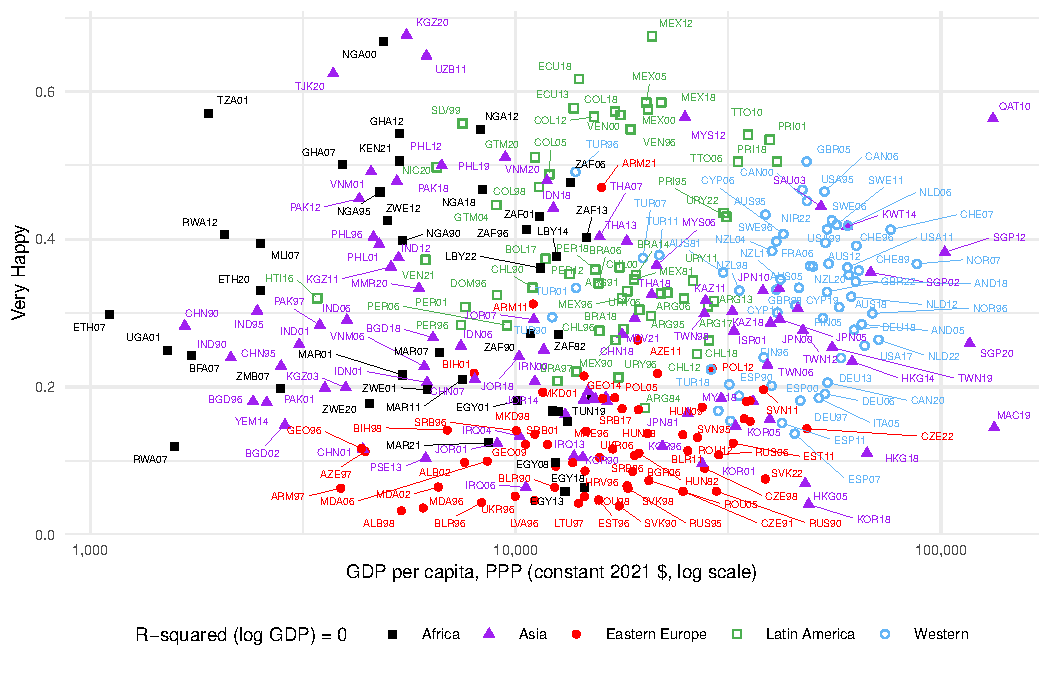
\includegraphics[width=.9\textwidth]{../figures/main/wvs_very_happy_vs_gdp_ppp.pdf}
\end{figure}

\begin{figure}[htbp]
    \centering
    \caption{Mean ladder vs.\ GDP per capita (PPP), Gallup, last observation per country}\label{fig:gallup_gdp}
    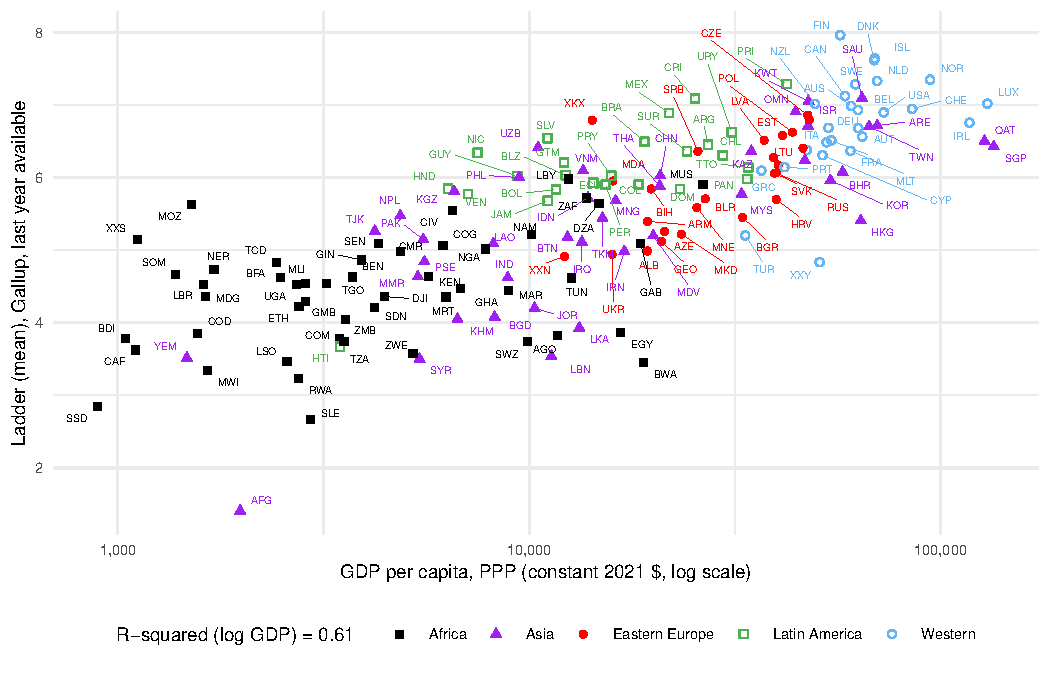
\includegraphics[width=.9\textwidth]{../figures/main/gallup_ladder_mean_vs_gdp_ppp.pdf}
\end{figure}


\end{document}
